\documentclass[journal,a4paper]{IEEEtran}
\usepackage{url}
\usepackage{graphicx, subfigure}

\title{ Software Weaknesses Detection using Static-code Analysis and Machine Learning Techniques}

\begin{document}
\pagestyle{empty}
\author{S. Conte$^a$, N. Leite$^b$, J. Simão$^b$\\
{$^a$Departamento de Engenharia de Electrónica e Telecomunicações e de Computadores, Instituto Superior de Engenharia de Lisboa, Portugal}\\
%{$^b$Other Department, Other University, Other Country}\\
\hspace{0.3cm} A43854@alunos.isel.pt \ nuno.leite@isel.pt \  jose.simao@isel.pt}

\maketitle

% Abstract.
\begin{abstract}
In the modern world, the software industry plays a pivotal role across various domains. Software vulnerabilities represent a significant threat to computer security. While there are tools to detect vulnerable code, their accuracy remains a challenge. Existing solutions often require expert manual input to define vulnerability features. The increasing number of security vulnerabilities is a growing concern, indicating a need for improved detection methods. This has led to the application of machine learning in software engineering and cybersecurity. Our work introduces a machine learning-based vulnerability detection system that utilizes static code analysis to extract code dependencies and generate data features. We collected data from the NIST SAMATE project, focusing on Java code with Null Pointer Dereference and Command Injection vulnerabilities. We used control flow graphs and data-flow analysis for feature extraction. Our tool demonstrated reduced false negatives with a manageable number of false positives. Additionally, we successfully applied the tool to real software products to identify vulnerabilities, despite some false positives.
\end{abstract}

% Keywords.
\vspace{.5cm}
\textbf{Keywords: control flow graph, Data-flow analysis, feature extraction, machine learning, reaching definitions, static-code analysis, vulnerability detection.}

% Section 1
\section{Introduction}

In today's context, the absence of software security presents a significant challenge for businesses and organizations. Software vulnerabilities not only lead to increased costs but can also be exploited by malicious actors, resulting in various degrees of harm to individuals and entities. It is essential to have the necessary tools and techniques for predicting and detecting vulnerabilities within software components created by development teams.
To address this issue, organizations like OWASP (Open Web Application Security Project) release informative documents aimed at raising awareness among developers and emphasizing web application security. Their latest standard, the "Top 10 Web Application Security Risks" published in 2021, documents the most critical vulnerabilities found in software \cite{OWASP_TOP_TEN2021}.
More recently, there has been a growing focus on applying machine learning techniques to enhance software security. One of the primary challenges in identifying vulnerabilities is the difficulty of extracting features that effectively describe vulnerable code and distinguish it from secure code. Various approaches to vulnerability detection have been explored \cite{Seyed_Hamid_2022}, including models based on software metrics, which consider high-level features such as code complexity, anomaly detection models, and the recognition of vulnerable code patterns.
Our contributions: In this study, we have explored the use of static code analysis combined with machine learning techniques to identify critical software security vulnerabilities. Subsequently, we implemented a prototype tool that utilizes these techniques to learn vulnerability features from a comprehensive database obtained from SAMATE \cite{SAMATE2023}. The prototype tool is specifically designed for the Java programming language and serves as a proof of concept, demonstrating the effectiveness of this approach in vulnerability detection. Its applicability highlights the potential of combining static code analysis and machine learning to detect vulnerabilities in source code.

\section{Related Work}

Kronjee et al. \cite{Kronjee2018} introduce an innovative approach to static analysis, wherein they combine data-flow analysis with machine learning techniques to identify vulnerabilities within source code \cite{Kronjee2018}.

They had investigated whether machine learning techniques in conjunction with static code analysis to identify insecure code within a particular dynamic programming language, specifically PHP. The focus of the research has been on web application vulnerabilities, specifically SQL injection (SQLi) and Cross-Site Scripting (XSS). They had tried to demonstrate that using machine learning in combination with features extracted from control-flow graphs and abstract syntax trees can be an effective approach for vulnerability detection in dynamic languages, in particular PHP applications.To demonstrate the effectiveness of their approach, they developed a tool called \texttt{WIRECAML} and assessed its performance against other vulnerability detection tools for PHP code. Nevertheless, the tool has its share of limitations, arising from both inherent and technical factors. The complexity of dealing with arrays of data and the presence of multiple vulnerabilities in various versions of the same application contribute to a notable issue in the dataset - duplicate samples.


Wartschinski et al. introduced VUDENC (Vulnerability Detection with Deep Learning on a Natural Codebase), a vulnerability detection system that utilizes deep learning to autonomously learn features from a vast collection of real-world code \cite{Wartschinski2019}. The main goal of VUDENC was to alleviate the labor-intensive and subjective process of manually defining features for vulnerability detection \cite{Wartschinski2019}. They gathered a substantial dataset of commits from GitHub, labeled based on the commit context. Data samples were generated from vulnerable code files, with a fine-grained analysis of individual code tokens and their context. They also employed a word2vec model to train on a large Python code corpus, enabling the creation of embeddings for code tokens that preserve semantics \cite{Wartschinski2019}.
The research effectively demonstrated the ability to use machine learning directly on source code to learn features related to vulnerabilities, employing LSTM models. VUDENC was tailored to work with Python source code and exhibited proficiency in predicting seven distinct types of vulnerabilities \cite{Wartschinski2019}.

Zhen Li et al. introduced VulDeePecker, the first deep learning-based vulnerability detection system \cite{Zhen_Li2018}. The system aimed to automate the feature definition process and reduce false negatives in vulnerability detection. They began by establishing guiding principles for applying deep learning to vulnerability detection since deep learning was not originally developed for this purpose. The authors also provided a valuable dataset for evaluating VulDeePecker and future deep learning-based vulnerability detection systems \cite{Zhen_Li2018}.

Despite its promising approach, VulDeePecker had several limitations in its design, implementation, and evaluation. It was primarily focused on vulnerability detection when source code was available, leaving the detection of vulnerabilities in executables as a more complex challenge. Additionally, VulDeePecker was designed to work specifically with C/C++ programs. Future research is necessary to adapt the system to handle other programming languages \cite{Zhen_Li2018}.

\section{Methodology}
In this section, we present the proposed architecture and the different steps followed to conduct the study.

\subsection{Proposed Architecture}

We proposed an approach inspired by a research that used data-flow analysis and machine learning to detect SQLi and XSS vulnerabilities in PHP software code \cite{Kronjee2018}. In the proposed architecture, presented in the Figure \ref{fig:archquitecture}, we opted for Java as the target programming language and chose to focus on detecting weaknesses such as NULL Pointer Deference and Command Injection.

\begin{figure*}
  \centering
  \includegraphics*[width=0.90\textwidth]{Architecture3}
  \caption{A high-level flow of proposed architecture.}
  \label{fig:archquitecture}
\end{figure*}

As depicted in Figure \ref{fig:archquitecture}, the project was organized into two main phases. The initial phase comprised dataset building, in which we generated Control Flow Graphs (CFGs) from Java source files and extracted corresponding features. Subsequently, the following phase involved learning and detection. During this phase, we divided the dataset into two subsets: the training set, designated for model training, and the testing set, used for model assessment.

We used reaching definition and taint analysis to identify potential vulnerabilities in the code. With the help of the Abstract Syntax Tree (AST), we determined if a variable was being used as a parameter in a function call. This allowed us to extract features by providing functions and their corresponding argument values (variables) to our probabilistic classifier. Through this method, our machine learning algorithm learned which functions were likely to be potentially vulnerable based on collected samples.

To determine if a function was applied to a variable, we constructed a Control Flow Graph (CFG) from the AST. By considering the entire preceding execution path, we used the invocation of functions in that path as a feature.

For efficient feature extraction, we utilized a parser capable of translating code into an AST and creating a Control Flow Graph. This was made possible using the "spoon-control-flow" component \cite{OW2_SPOON}, which could generate both control-flow and data-flow graphs for Java programs based on its AST created using the Spoon library. We implemented reaching definitions analysis and use-definition techniques to extract features from the AST.

\subsection{Data Preparation}

This section corresponds to the first phase in the proposed architecture. Describes all the implementation done about this part of architecture.

Before developing the tool, the initial step was to gather a substantial number of Java projects relevant to our case study on vulnerabilities, specifically NPD and CI. To effectively address these vulnerabilities, we needed a diverse set of examples for each type.

The NIST Software Assurance Metrics And Tool Evaluation (SAMATE) project maintains numerous test cases for various programming languages and vulnerability types. These test cases are built on the Common Vulnerabilities and Exposures (CVE) standard vulnerability dictionary \cite{CVE_2023}. SAMATE categorizes vulnerabilities according to the Common Weakness Enumeration (CWE) \cite{CVE476}, and it includes Java test cases for command injection and Null Pointer Dereference vulnerabilities. We were able to filter and acquire 800 projects for CI and 600 projects for NPD. Each project was downloaded from SAMATE to our local machine for further processing.

On the other hand, the National Vulnerability Database (NVD) doesn't store vulnerable source code projects but rather provides information on reported vulnerabilities along with relevant links. However, this information isn't organized in the same way as SAMATE's. Extracting data from NVD would have required additional effort, such as creating our own list of Java projects from various sources, and manually identifying vulnerable projects through search. Due to these challenges, we couldn't utilize NVD, and we consider this task for future work.

To process and create the dataset from SAMATE data, each Java project went through a series of transformations. First, the project was converted to an Abstract Syntax Tree (AST) using the Spoon library. Subsequently, all elements of the AST related to functions were filtered. Then, each function was represented as a Control Flow Graph (CFG) to facilitate data-flow analysis.

In the dataset, the invoked methods corresponded to the feature "Func," while the values of the arguments passed to these methods were captured as the feature "Var." The model learned whether functions were vulnerable based on the argument values passed to them. The resulting dataset was saved in a CSV file.

\subsection{Model Creation}

This section corresponds to the second phase of the proposed architecture. Once we have the dataset created and ready to be used in training, we are able to create the model. The next list describes the entire implementation process.

These are the steps followed during the model creation process:

\begin{enumerate}
\item Tokenizing text data

To perform machine learning on text data, it's necessary to convert the text content into numerical feature vectors \cite{Text_Data}. This process involves assigning a unique number to each word, effectively encoding the text data into fixed-length vectors, with each position in the vector representing a word from the vocabulary. The value at each position can indicate the count or frequency of the corresponding word in the document.

\item Using Synthetic Minority Oversampling Technique (SMOTE) for imbalanced classification data

Our model's training data had an imbalance, with a bias toward the majority class, making it challenging for the model to make accurate predictions for the minority class. This resulted in classification algorithms favoring the majority class and performing poorly on the minority class.

To address this issue, we implemented oversampling for the minority class (vulnerable class). We achieved this by duplicating examples from the minority class in the dataset before training the model by using smote technique  \cite{chawla2002smote}. This balanced the class distribution without introducing any new information to the model.

\item Splitting dataset into training and validation set

After converting our text data into numerical feature vectors and balancing the class distribution using SMOTE, we proceeded to split the dataset into the following subsets:
Training Set: This subset was utilized to train the machine learning model. The model learned patterns and features from the training data, enabling it to make predictions on new, unseen data.
Test Set: The Test set served as a means to assess the performance of the trained model. It mimicked new, unseen data and allowed us to evaluate how well the model generalized to unfamiliar examples.

\item Using K-fold cross-validation

K-fold cross-validation is a common technique for assessing a model's performance. It entails splitting the dataset into k equal parts or folds and repeatedly training and evaluating the model. In each iteration, one fold serves as the test set while the remaining folds act as the training set. This process repeats ten times to ensure each fold serves as the test set once. The results from these evaluations are then averaged to provide a more robust and reliable performance estimate for the model \cite{inbook_Cross_Validation}.

The primary reason for employing k-fold cross-validation is its simplicity, ease of implementation, and its tendency to produce less biased estimates when compared to other methods. Additionally, it offers the advantage of random data partitioning.

\item Build multiple different models to predict vulnerability from our dataset

Since we didn't know which algorithms would be good for our problem or what configurations to use, we had to create different models using various algorithms.

We used a mixture of simple linear, nonlinear algorithms. We decided to also use deep learning (Multi-layer Perceptron classifier) to make a small experiment. The followings are algorithms used on the process: Logistic Regression (LR), Decision Tree (DT), Neighbor Classifier (NC), Naive Bayes (NB), Support Vector Machines (SVM), Multi-layer Perceptron classifier (MLPC) - Deep Learning.

\item Select the best model as our final model

Following the construction and evaluation of various models, we conducted a comparative analysis to determine the most accurate model, which was chosen as our final model. Subsequently, we used the validation dataset to assess the final model's accuracy. The final model was trained on the complete training dataset, and predictions were generated for the validation dataset. To evaluate these predictions, we compared them to the expected outcomes in the validation set. Our evaluation included the calculation of classification accuracy, the creation of a confusion matrix, and the generation of a classification report. Detailed experimental results are provided in the following section.
\end{enumerate}

\section{Experiments and Discussion}

The models were trained on the training datasets, and their performance was evaluated with the validation dataset. This section describes the experimental results obtained during the evaluation with the test set.

The prediction result of the model can fall into one of four categories: True Positive (TP), True Negative (TN), False Positive (FP), and False Negative (FN). From the counts of TP, TN, FP, and FN, various performance indicators can be calculated, including precision, F1-score, Brier Score, and others. These metrics provide a comprehensive understanding of the model's performance and can guide further optimization.

\subsection{Model Performance}

We made a chart to evaluate the models, comparing how the accuracy results vary between different models. We tested each model 10 times using a technique called 10-fold cross-validation, which helps ensure our results are reliable.

For Command injection vulnerability data, we used 60\% for training (7,872 samples) and 40\% for testing (5,248 samples). We made sure the split kept the same proportion of target classes in both sets.
For Null Pointer Dereference vulnerability, we had 1,046 samples for training and 764 samples for testing.

The results are presented Tables \ref{tab:results_probabilistic_classifiers_NPD}, \ref{tab:results_probabilistic_classifiers_CI}. 


\begin{table*}[!ht]
    \centering
    \caption{Statistical summary of average performance among different probabilistic classifiers for Null Pointer Deference.}
    \begin{tabular}{|l|l|l|}
    \hline
        \textbf{Vulnerability Type} & \multicolumn{2}{|c|}{\textbf{Null Pointer Deference}} \\ \hline
        Classification method &  mean accuracy & Standard deviation Accuracy \\ \hline
        Logistic regression & 0.996154 & 0.007692 \\ \hline
        Decision tree & 0.923385 & 0.024098 \\ \hline
        Support vector machines & 0.996154 & 0.007692 \\ \hline
        Naive Bayes & 0.996154 & 0.007692 \\ \hline
        Neighbor classifier & 0.996154 & 0.007692 \\ \hline
        Multi-layer Perceptron classifier & 0.999846 & 0.000462 \\ \hline
    \end{tabular}
	\label{tab:results_probabilistic_classifiers_NPD}
\end{table*}

\begin{table*}[!ht]
    \centering
    \caption{Statistical summary of average performance among different probabilistic classifiers for Command Injection.}
    \begin{tabular}{|l|l|l|}
    \hline
        \textbf{Vulnerability Type} & \multicolumn{2}{|c|}{\textbf{Command Injection}} \\ \hline
        Classification method &  Mean Accuracy & Standard deviation Accuracy \\ \hline
        Logistic regression & 0.998096 & 0.001528 \\ \hline
        Decision tree & 0.94919 & 0.008034 \\ \hline
        Support vector machines & 0.999873 & 0.000381 \\ \hline
        Naive Bayes & 0.999873 & 0.000381 \\ \hline
        Neighbor classifier & 0.999873 & 0.000381 \\ \hline
        Multi-layer Perceptron classifier & 0.999772 & 0.000684 \\ \hline
    \end{tabular}
	\label{tab:results_probabilistic_classifiers_CI}
\end{table*}

Tables \ref{tab:results_probabilistic_classifiers_NPD}  and \ref{tab:results_probabilistic_classifiers_CI} show the results of the mean and standard deviation accuracy of the several probabilistic classifiers for Null Pointer Deference and Command Injection vulnerabilities.

%\begin{figure*}
%\centering     %%% not \center
%\subfigure[CI vulnerability]%{\label{fig:Plot_ML_CI_FIG}\includegraphics[width=\textwidth]%%$%{Plot_ML_CI}}
%\subfigure[NPD vulnerability]%{\label{fig:Plot_ML_CI_NPD}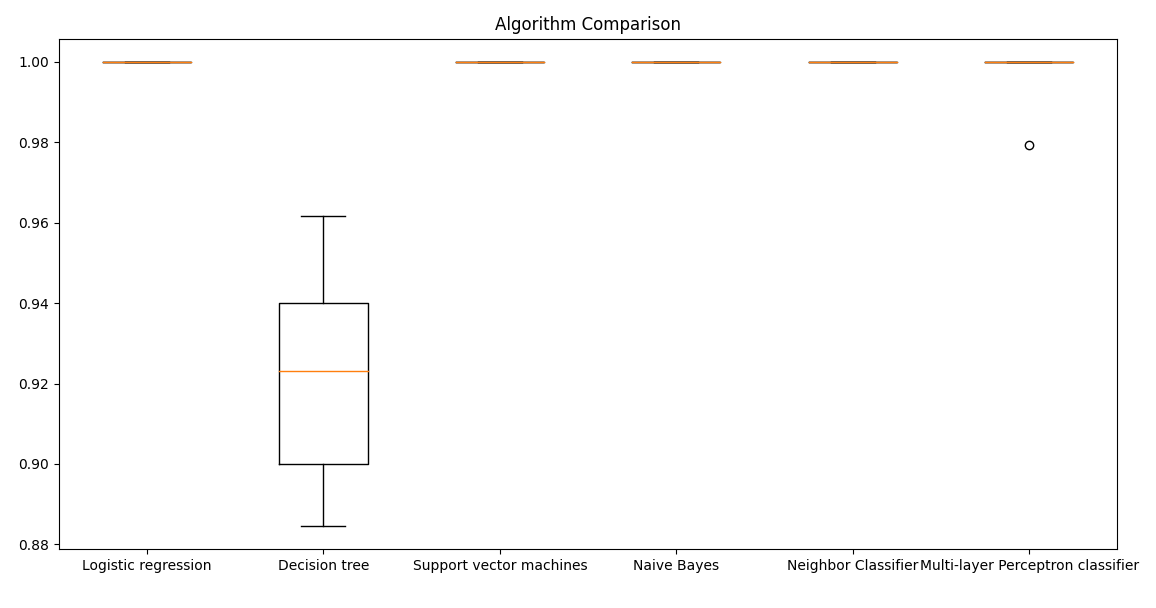
\includegraphics[width=\textwidth]{Plot_ML_NPD}}
%\caption{Box and Whisker Plot Comparing Machine Learning Algorithms for NPD and CI vulnerability}
% \label{fig:Plot_ML_BOX_FIG}
%\end{figure*}

%The figures \ref{fig:Plot_ML_CI_FIG} and \ref{fig:Plot_ML_CI_NPD} show the result of cross val score method  execution, which calculates the accuracy for each algorithm.

%Figures \ref{fig:Plot_ML_CI_FIG} and \ref{fig:Plot_ML_CI_NPD} show the box and whisker plots for each model, using the accuracy measure. Therefore, LR, NB, SVM, NC, and MPLC are the best algorithms for our dataset, as the figure \ref{fig:Plot_ML_BOX_FIG} illustrates. There are more options in choosing algorithms, which is beneficial for our model.

%We can see in the Figure \ref{fig:Plot_ML_BOX_FIG} that the box and whisker plots are squashed at the top of the range, with many evaluations achieving almost 100\% accuracy, and some pushing down into the high 90\% accuracy (in case of Decision Tree).

Tables \ref{tab:results_probabilistic_classifiers_NPD}  and \ref{tab:results_probabilistic_classifiers_CI} show the result of cross val score method  execution, which calculates the accuracy for each algorithm. Therefore, LR, NB, SVM, NC, and MPLC are the best algorithms for our dataset. There are more options in choosing algorithms, which is beneficial for our model.

Given that there are several algorithms with good accuracy, we choose Logistic Regression to use in our final model. Next, the evaluation results obtained with the test set are presented for each type of vulnerability.

\begin{figure*}
\centering     %%% not \center
\subfigure[NPD vulnerability]{\label{fig:ConfusionMatrix_NPD_FIG}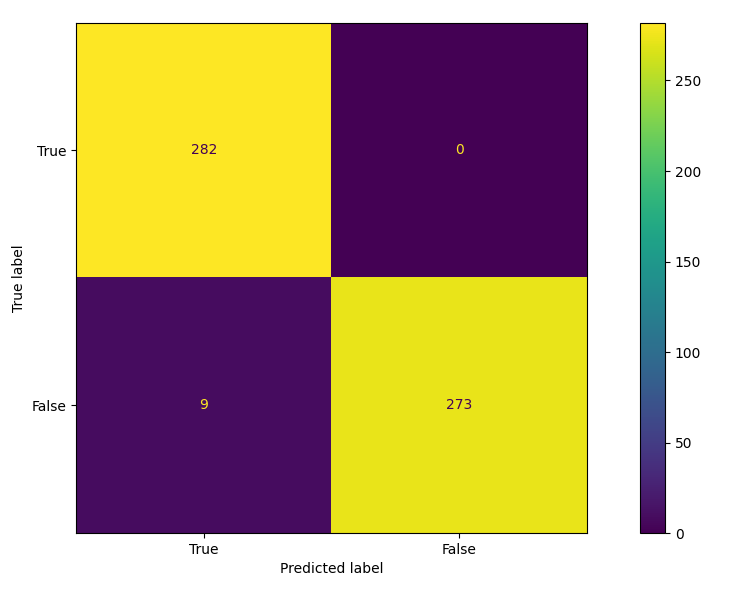
\includegraphics[width=9cm]{ConfusionMatrix_NPD2}}
\subfigure[CI vulnerability]{\label{fig:ConfusionMatrix_CI_FIG}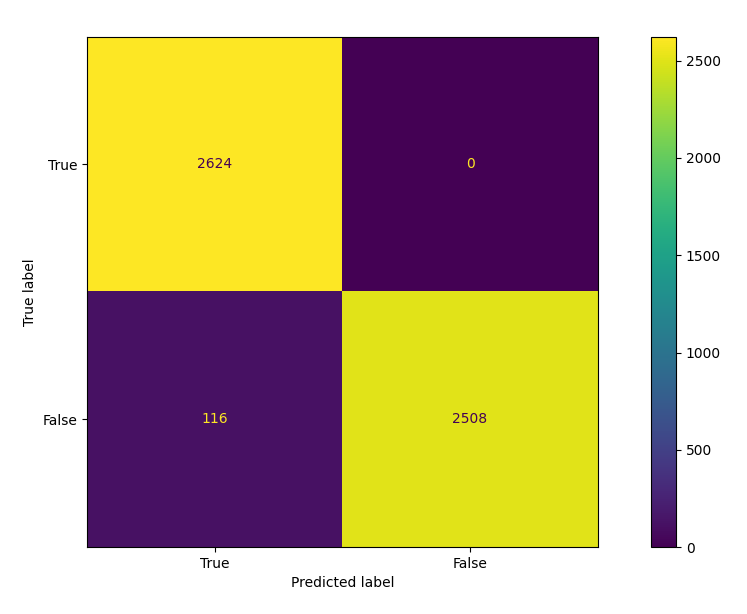
\includegraphics[width=9cm]{ConfusionMatrix_CI2}}
\caption{Comparing LR model confusion matrix for ND and CI vulnerability}
\end{figure*}

The figures \ref{fig:ConfusionMatrix_NPD_FIG} and \ref{fig:ConfusionMatrix_CI_FIG} show the confusion matrix results for the LR models for both vulnerabilities, illustrating the true and predicted classifications for our test set.

\begin{figure*}
\centering     %%% not \center
\subfigure[NPD vulnerability]{\label{fig:PrecisionRecall_NPD_FIG}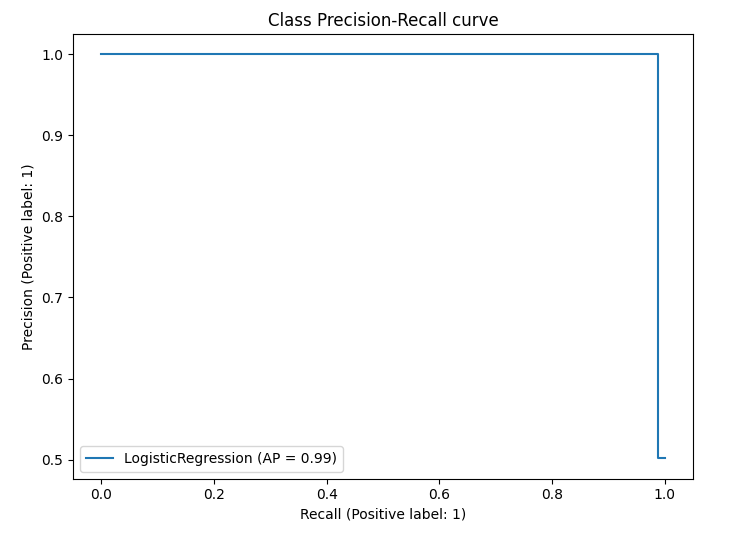
\includegraphics[width=9cm]{PrecisionRecall_NPD}}
\subfigure[CI vulnerability]{\label{fig:PrecisionRecall_CI_FIG}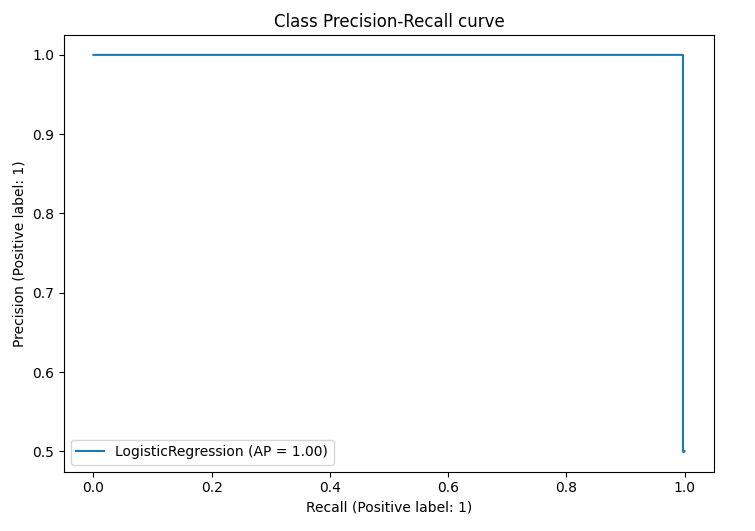
\includegraphics[width=9cm]{PrecisionRecall_CI}}
\caption{LR model Precision-Recall Plot for NPD and CI vulnerability}
\end{figure*}


The precision-recall curve is depicted in Figures \ref{fig:PrecisionRecall_NPD_FIG} and \ref{fig:PrecisionRecall_CI_FIG}, illustrating the precision and recall for different thresholds in the logistic regression model. In this graph, recall is on the x-axis, and precision is on the y-axis.

When the Area Precision is 0.99, closer to 1, it indicates that the model has a good balance between precision and recall, effectively classifying instances while minimizing false positives.

Figure \ref{fig:ClassificationReportCI_NPD_FIG} illustrates different classification metrics provided by scikit-learn tool's classification reports, detailing how well the model is performing on different classes.

\begin{figure*}
\centering     %%% not \center
\subfigure[NPD vulnerability]{\label{fig:ClassificationReportNPD_FIG}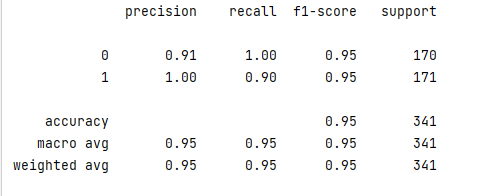
\includegraphics[width=9cm]{ClassificationReportNPD}}
\subfigure[CI vulnerability]{\label{fig:ClassificationReportCI_FIG}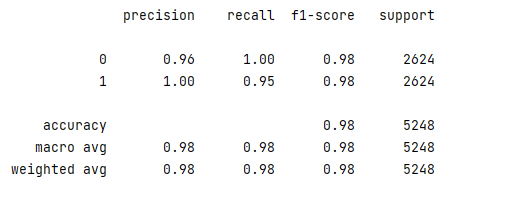
\includegraphics[width=9cm]{ClassificationReportCI}}
\caption{Comparing LR classification report for NPD and CI vulnerability}
\label{fig:ClassificationReportCI_NPD_FIG}
\end{figure*}

Figures \ref{fig:ClassificationReportNPD_FIG} and \ref{fig:ClassificationReportCI_FIG} show the classification report for different metrics such as precision, recall, F1-score, and support. The results show a high rate of these metrics for both vulnerable and not-vulnerable instances despite of false positive cases.

Discussion: In this the models demonstrated strong performance for both types of vulnerabilities. However, there were a few instances of false negatives where the model didn't correctly identify certain functions that were, in fact, vulnerable.

We also observed a significant number of false positives, which implies that the model effectively recognized all non-vulnerable functions. However, we will later uncover that this high number is misleading when testing the model with data from other projects. This discrepancy arises because certain functions, though seemingly non-vulnerable, receive arguments with patterns identical to those of vulnerable functions

Further refinement of the 'Var' attribute is essential to precisely match the pattern with the actual vulnerable code, ideally using the same string. This is necessary because each project specifies values differently, which differs from how SAMATE projects do it.

We've reached the conclusion that we have effective models for both types of vulnerabilities, showing strong performance. Despite a few instances of false positives, our models successfully identified vulnerabilities in genuinely vulnerable areas.aces.

\subsection{Model Evaluation with data from other projects}

Given the good results with samate data, we decided to analyse if our tool could detect vulnerabilities from real software projects.

We searched for some examples of vulnerable Java code on GitHub and found the following projects for Command injection vulnerability: Vulnerable Java Application \cite{github_Christophe}, Java Sec Code \cite{github_Syclover}, Operation System Command Injection Vulnerability in Java Spring \cite{github_Will}, Amaze File Manager \cite{github_Vishal}, OpenTSDB 2.4.0 Remote Code Execution \cite{github_Chris}, OS Command Injection \cite{github_Utku}, and the following projects for Null Pointer Deference vulnerability: null-pointer-dereference-examples \cite{github_Sridhar}, Selenium \cite{github_Harsha} and dbus-java \cite{github_David}.

For each project, we used our dataset generator tool to transform the source code into a dataset through feature extraction. This was achieved by providing the project directory path to the tool. Subsequently, we applied the models trained with SAMATE data to identify vulnerabilities. The tool generated a CSV file for each project, including details like file name, line number, node number, and probability for each instance. We confirmed the presence of vulnerabilities through manual inspection.

The results are resumed in Tables \ref{tab:model_evaluation_results_CI} and \ref{tab:model_evaluation_results_NPD}. The "Project" field indicates the name of the project. The "Vuln. Lines" indicates the number of vulnerable lines predicted by the model. The "Non-Vul. Lines" indicates the number of non-vulnerable lines predicted by the model. The "Tot. lines" indicates the total number of lines extracted from the project. The "Comments" provides a qualitative assessment of the model's behavior in that project. 

\begin{table*}[!ht]
    \centering
    \caption{Result of model evaluation  using real software projects for command injection vulnerability.}
    \begin{tabular}{|p{1.5in}|p{0.5in}|p{0.5in}|p{0.5in}|p{3in}|}
    \hline
        \textbf{Project} & \textbf{Vuln. Lines} & \textbf{Non-Vul Lines} & \textbf{Tot. lines } & \textbf{Comments} \\ \hline
        Vulnerable Java Application & 1 & 5 & 6 & Predicted correctly. The prediction was consistent. \\ \hline
        Java Sec Code & 20 & 218 & 238 & Incorrectly predicted. The prediction was inconsistent. \\ \hline
        OS Command Injection Vulnerability in Java Spring & 0 & 1 & 1 & In this project, it was only possible to extract one line to create the dataset, which is actually vulnerable. Unfortunately, the model missed it. The prediction was inconsistent. \\ \hline
        ArmazeFileManager & 116 & 1090 & 1206 & The model was able to detect the vulnerable functions. The prediction was inconsistent. \\ \hline
        OpenTSDB 2.4.0 Remote Code Execution & 220 & 2085 & 2305 & The model was able to detect the vulnerability, but the prediction was inconsistent. \\ \hline
        OS Command Injection & 0 & 3 & 3 & Incorrectly predicted. The prediction was inconsistent. \\ \hline
    \end{tabular}
	\label{tab:model_evaluation_results_CI}
\end{table*}

\begin{table*}[!ht]
    \centering
    \caption{Result of model evaluation  using real software projects for Null Pointer Deference vulnerability.}
    \begin{tabular}{|p{1.5in}|p{0.5in}|p{0.5in}|p{0.5in}|p{3in}|}
    \hline
        \textbf{Project} & \textbf{Vuln. Lines} & \textbf{Non-Vul Lines} & \textbf{Tot. lines } & \textbf{Comments} \\ \hline
        null-pointer-dereference & 25 & 160 & 185 & The model was able to detect the vulnerability, but the prediction was inconsistent. \\ \hline
        dbus-java & 38 & 238 & 276 & Incorrectly predicted. the prediction was inconsistent. \\ \hline
        SeleniumHQ & 70 & 1149 & 1219 & The model was able to detect vulnerable lines, but the prediction was inconsistent. \\ \hline
    \end{tabular}
	\label{tab:model_evaluation_results_NPD}
\end{table*}

As shown in the tables \ref{tab:model_evaluation_results_CI} and \ref{tab:model_evaluation_results_NPD} and explained earlier, The model is also finding vulnerabilities (false positives) in functions that receive variables, which might come from user input or be null, making them appear tainted, but these functions are not actually vulnerable. In some cases, the functions don't even receive any arguments, so identifying them as vulnerable doesn't make sense.

Discussion: Based on this analysis, we can observe that in a significant number of projects, the models predictions were inconsistent, meaning they tend to be less stable (predicting some instances incorrectly). Nevertheless, it's worth noting that the models were successful in detecting vulnerabilities in certain projects. We recognize the need for further refining the 'Var' feature to precisely align its pattern with the actual vulnerable code, ideally matching the same string. Even when the commands themselves are identical, each project defines its unique path for command execution. In essence, we suspect that the 'Var' feature's value in the SAMATE dataset differs from the actual code, primarily due to the distinct nature of each project. This disparity notably impacts vulnerability detection. Due to time constraints, this couldn't be done, and therefore, it remains for future work.

\subsection{Comparison with other works}

This section consists of comparisons with similar works in the field to provide a perspective from which observations and measurements are made for the evaluation of this work. As there are fundamental differences in each approach, and direct comparison cannot be drawn between the outcomes. The current design of our tool is limited to Java programs. Future research should be conducted to adapt it for use with other programming languages.

Discovering vulnerabilities using data-flow analysis and machine learning: This is the main work related to our problem. It combines static code analysis with machine learning for detecting SQL injection (SQLi) and Cross-Site Scripting (XSS) vulnerabilities in PHP applications. It also uses SAMATE for collecting training data for the model \cite{Kronjee2018}.

The study aimed to demonstrate the potential of combining machine learning with static code analysis for software vulnerability detection. However, the results showed some uncertain, particularly when the tool was tested with different data sources (data from other applications). The absence of demonstrated data extracted from other projects for testing raises concerns. Specifically, the study did not provide evidence of the data used to evaluate their tool's performance. Additionally, our analysis suggests that the feature extraction process and dataset creation method heavily rely on function names, leading to varying features across different projects. The inconsistency in feature size and function names could limit the applicability of the model created and trained with a specific dataset (e.g., SAMATE data) to other datasets from different projects or source codes. As a result, the study's findings may not be considered definitive.

VUDENC - Vulnerability Detection with Deep Learning on a Natural Codebase: It is a vulnerability detection system that utilizes neural networks to learn vulnerable features from a collection of data extracted from GitHub. The work focuses on the Python programming language and exclusively learns source code \cite{Wartschinski2019}.
This work managed to demonstrate the potential use of deep learning directly on source code to learn vulnerable features, utilizing LSTM (Long Short-term Memory) models \cite{article_LSTM}.
They created the model using LSTM and managed to achieve good results. With an F1 score of around 87\%, they attained a precision of 91\% and a recall of 83\%.
Their tool was able to detect several types of vulnerabilities, and this is the main advantage of their work compared to ours. Another advantage in comparison with our approach is that they used real GitHub data for model creation. In our case, we used SAMATE data for training and model creation.

VulDeePecker Deep Learning Based System For Vulnerability Detection: Li et al. \cite{Zhen_Li2018} developed this tool  to detect buffer error vulnerabilities and resource management error vulnerabilities in C/C++ programs. They used a 'code gadget database' from popular open source projects like Linux kernel and Firefox. They found vulnerabilities using NVD and SAMATE datasets, which include synthetic and real-world code flaws. Like us, they gathered projects with vulnerable code to create a dataset and manually labeled the vulnerable parts. However, our approach automates this process (Our tool automates the process of labelling the vulnerable codes).

The authors of VulDeePecker compared their tool to other approaches and found a precision of 25\% for the Flawfinder  tool \cite{Flawfinder_}, 39.6\% for Checkmarx \cite{Checkmarx_}, and 19.4\% for RATS \cite{RATS_}, in contrast to VulDeePecker's precision of 88.1\%. Which means that VulDeePecker is more effective than these tool. The VulDeePecker approach successfully was able to reduce the number of false positive results to almost zero, a level of achievement that we were unable to accomplish in our case.

\subsection{Limitations}

The current design, implementation, and evaluation of this work have some limitations that point to potential areas for future research. Firstly, this work design is primarily limited to address various vulnerability types. The feature extraction process represents challenges for projects compatible with Java programming language version 8 and beyond, particularly when dealing with functional programming paradigms like lambda expressions in feature extraction.

Second, the present design of our tool only deals with Java programs. Future research needs to be conducted to adapt it to deal with other kinds of programming languages.

Third, the present design of this work only deals with vulnerabilities related to functions invocation. The future work could investigate how to detect the other kinds of vulnerabilities by leveraging the other kinds of key points.

Fourth, The data collected for model creation was just from one source (SAMATE) and  insufficient, it's necessary to collect more data from different sources and from real example source code.

Fifth, we evaluated the model's performance using standard measures commonly used in vulnerability prediction, like predictions, accuracy, precision, and recall. While we used common and accepted measures, there might be other metrics worth exploring to assess how well the classifier performs.

Sixth, currently, our tool only uses machine learning classifiers. To improve our experiments, we can try different techniques like Natural Language Processing, Recurrent Neural Networks, and Convolutional Neural Networks (CNNs). We might also combine these methods for a more complete approach.

Seventh, Another limitation is that we didn't fine-tune our model's hyperparameters. Hyperparameter tuning helps optimize a machine learning model, making it perform better.

Finally, furthermore, design decisions were made which might affect the overall end result.

\section{Conclusion and Future Work}

In this work, we introduced a system that uses Machine Learning to find vulnerabilities in source code. Our goal is to make it easier and less subjective than having humans manually define what makes code vulnerable. This study shows that machine learning can learn from source code to detect vulnerabilities by using classifier models.

The system focuses on Java source code and can predict two types of vulnerabilities: Command Injection and Null Pointer Dereferences. We built the tool's foundation using a substantial dataset from SAMATE projects, which was adjusted to match the model's requirements. This data came from various SAMATE projects and included code snippets for both vulnerability types.

A classifier model based on Logistic Regression algorithm has been trained on a large data of java source code to be able to perform vulnerabilities detection. Systematic experiments show that our tool achieves, on average, an accuracy of 96.5\%, a recall of 95\%, a precision of 95\% and an F1 score of 96.5\% using SAMATE data with a ratio of 60\% for the training dataset and 40\% for the test dataset. Similarly, with data from real projects, we achieved favorable results. Despite encountering some false positives, the model was able to detect vulnerabilities in genuinely vulnerable locations. These results are very promising and encourage for further research in this area.

\subsection{Future Work}

There are several unsolved issues for future research in this field of study. Firstly, the approach itself could probably be adjusted and improved, for instance, by optimizing the feature extraction process or more data collection as discussed earlier.

The 'Var' attribute values could be refined in order to match exactly the same pattern with the truly vulnerable codes In order to improve false positives cases from the model.

Our dataset is biased because we have many more non-vulnerable code lines than vulnerable ones. To improve this, we can compile and filter the data more carefully to get better samples. By collecting data from various sources, we can make sure we have a higher percentage of relevant examples.

Our approach could be experimented with different programming languages like PHP, C++, or C\#. First, we need to see if the process of extracting features (data transformation) works well for those languages. If it does, we can train the model on datasets from those languages and compare it to other research. Additionally, we could use our approach on various types of applications, including web and mobile apps or software in specific fields with their unique security risks.

Finally, a subsequent expansion could involve building a fully functional vulnerability detection system with high usability that takes code as input and detect vulnerabilities. While a simple prototype tool has already been constructed in this work, it has not been optimized for usability in daily programming. One option would be to create a plugin for an IDE or a highly customized command line tool.

\section{Acknowledgment}

We would like to thank the anonymous reviewers
for their insightful comments and suggestions that would help us improve the article.

\small
\bibliographystyle{plain} 
\bibliography{i-etc-bib}

%\renewcommand{\baselinestretch}{0.98}
%\bibliographystyle{plain}
%{\small
%\bibliography{cetc-bib}}
%\renewcommand{\baselinestretch}{1}


\end{document}
